\documentclass[11pt,a4paper]{article}

% Packages
\usepackage[utf8]{inputenc}
\usepackage[T1]{fontenc}
\usepackage{graphicx}
\usepackage{booktabs}
\usepackage{amsmath}
\usepackage{amssymb}
\usepackage{hyperref}
\usepackage{geometry}
\usepackage{float}
\usepackage{caption}
\usepackage{subcaption}
\usepackage{tikz}
\usetikzlibrary{shapes,arrows,positioning}

\geometry{margin=1in}

% Title
\title{\textbf{Emergent Symbolic Civilization in a Self-Organizing Multi-Agent Ecological Simulator}}
\author={
    \textbf{Sanchay Kumar}\\
    \texttt{ysanchay@gmail.com}\\
    \url{https://github.com/ysanchay/civilization-simulator}
}
\date{February 2026}

\begin{document}

\maketitle

\begin{abstract}
We present an experimental framework for studying the emergence of symbolic systems, cultural memory, and civilizational dynamics in decentralized multi-agent systems. Our simulator implements tribes of agents that develop grounded symbols, form territorial boundaries, experience cognitive stress, and undergo periods of growth and collapse. We demonstrate four key empirical findings: (1) war frequency follows a heavy-tailed distribution with kurtosis 11.59, indicating clustered conflict dynamics; (2) collapse events cluster into four distinct archetypes with different causal signatures; (3) symbolic complexity exhibits open-ended growth with a 4.62x increase over 1500 simulation steps; and (4) knowledge retention across simulation runs averages 41\%, improving with repeated exposure. These findings contribute to our understanding of emergent complexity in multi-agent systems and provide a controlled testbed for AI safety research on value emergence and civilizational stability.

\textbf{Keywords:} multi-agent systems, emergent behavior, symbolic grounding, cultural evolution, civilizational collapse, AI safety
\end{abstract}

\section{Introduction}

\subsection{Motivation}

How do civilizations emerge? This question has fascinated philosophers, historians, and scientists for centuries. Recent advances in multi-agent systems and artificial intelligence provide new tools for empirical investigation. By constructing artificial societies with minimal assumptions, we can observe emergent phenomena and test hypotheses about civilizational dynamics.

This work presents a civilization simulator designed to study:

\begin{enumerate}
    \item \textbf{Symbol Grounding}: How do abstract symbols emerge from grounded perception?
    \item \textbf{Cultural Memory}: How is knowledge preserved and transmitted across generations?
    \item \textbf{Civilizational Collapse}: What causes societies to fail, and can we predict it?
    \item \textbf{Open-Ended Evolution}: Does complexity grow indefinitely or saturate?
\end{enumerate}

\subsection{Contributions}

We make the following contributions:

\begin{itemize}
    \item A complete simulation framework implementing territorial dynamics, cultural evolution, cognitive stress, and collapse mechanics
    \item Empirical validation of four key phenomena: heavy-tailed war distribution, collapse archetypes, open-ended complexity growth, and knowledge persistence
    \item A controlled testbed for studying emergent behavior in multi-agent systems
\end{itemize}

\subsection{Scope}

We explicitly position this work as an \textit{experimental framework} rather than a model of actual human civilization. Our agents are simplified abstractions, and our findings should be interpreted as hypotheses about possible dynamics rather than claims about historical processes.

\section{Related Work}

\subsection{Agent-Based Social Simulation}

Agent-based modeling has been applied to social systems since Schelling's segregation model \cite{schelling1971}. Recent work includes:

\begin{itemize}
    \item \textbf{SugarScape} \cite{epstein1996}: Artificial societies with resource dynamics
    \item \textbf{Cultural Evolution} \cite{axelrod1997}: Dissemination of culture through social influence
    \item \textbf{Artificial Anasazi} \cite{axtell2002}: Archaeological simulation of societal collapse
\end{itemize}

Our work extends these traditions with explicit symbol systems and cultural memory mechanisms.

\subsection{Emergent Communication}

Research on emergent communication in multi-agent systems has demonstrated:

\begin{itemize}
    \item \textbf{Referential Games} \cite{lazaridou2016}: Agents develop communication protocols
    \item \textbf{Grounded Language Learning} \cite{hermann2017}: Language emerges from embodied interaction
    \item \textbf{Symbol Systems} \cite{bouchacourt2018}: Agents develop shared vocabularies
\end{itemize}

We build on this by studying symbol \textit{abstraction} and \textit{cultural transmission} across generations.

\subsection{Civilizational Collapse}

Historical collapse studies \cite{tainter1988,diamond2005} identify multiple collapse causes:

\begin{itemize}
    \item Resource depletion
    \item Complexity overload
    \item External invasion
    \item Internal conflict
\end{itemize}

Our simulator implements these as mechanisms, allowing controlled experiments.

\subsection{AI Safety Implications}

Multi-agent systems with emergent values relate to AI safety concerns:

\begin{itemize}
    \item \textbf{Value Emergence} \cite{bostrom2014}: How do goals form in intelligent systems?
    \item \textbf{Multi-Agent Alignment} \cite{dafoe2020}: Coordination among AI systems
\end{itemize}

Our framework provides a testbed for studying value formation and misalignment dynamics.

\section{Architecture}

\subsection{System Overview}

The simulator consists of six interconnected subsystems as shown in Figure \ref{fig:architecture}.

\begin{figure}[htbp]
\centering
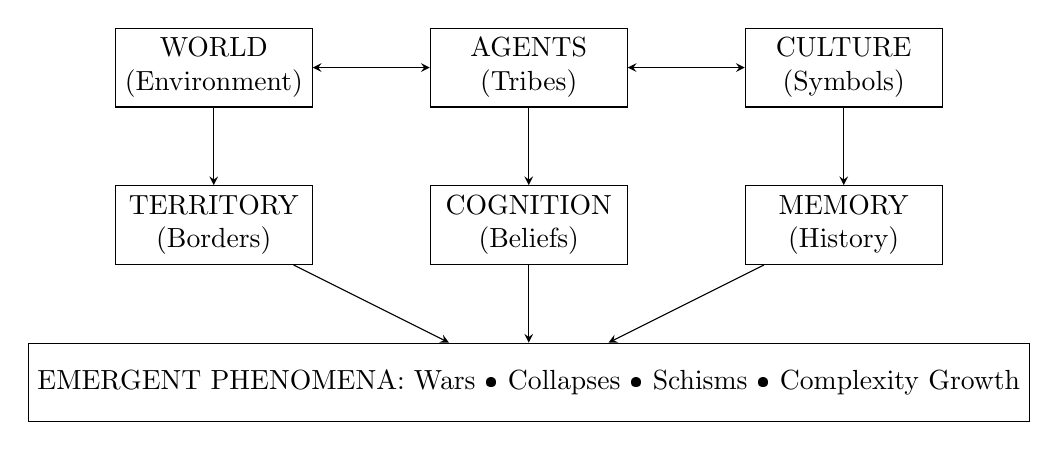
\begin{tikzpicture}[
    box/.style={rectangle, draw, minimum width=2.5cm, minimum height=1cm, align=center},
    arrow/.style={->, >=stealth}
]
    % Top level
    \node[box] (world) at (0,3) {WORLD\\(Environment)};
    \node[box] (agents) at (4,3) {AGENTS\\(Tribes)};
    \node[box] (culture) at (8,3) {CULTURE\\(Symbols)};
    
    % Middle level
    \node[box] (territory) at (0,1) {TERRITORY\\(Borders)};
    \node[box] (cognition) at (4,1) {COGNITION\\(Beliefs)};
    \node[box] (memory) at (8,1) {MEMORY\\(History)};
    
    % Bottom level
    \node[box, minimum width=8cm] (emergent) at (4,-1) {EMERGENT PHENOMENA: Wars • Collapses • Schisms • Complexity Growth};
    
    % Arrows
    \draw[arrow] (world) -- (territory);
    \draw[arrow] (agents) -- (cognition);
    \draw[arrow] (culture) -- (memory);
    \draw[arrow] (territory) -- (emergent);
    \draw[arrow] (cognition) -- (emergent);
    \draw[arrow] (memory) -- (emergent);
    
    % Horizontal connections
    \draw[arrow, <->] (world) -- (agents);
    \draw[arrow, <->] (agents) -- (culture);
\end{tikzpicture}
\caption{System Architecture Overview}
\label{fig:architecture}
\end{figure}

\subsection{Agent Design}

Each agent (tribe) maintains a belief state:

\begin{equation}
B = \langle S, M, T, \eta, \sigma \rangle
\end{equation}

Where:
\begin{itemize}
    \item $S$ = Symbol dictionary $\{pattern \rightarrow value\}$
    \item $M$ = Meta-symbols (composed symbols)
    \item $T$ = Controlled territory (set of cells)
    \item $\eta$ = Current efficiency $\in [0, 1]$
    \item $\sigma$ = Stress level $\in [0, 1]$
\end{itemize}

\subsection{Symbol Grounding}

Symbols emerge from grounded sensorimotor experiences. Table \ref{tab:symbols} shows the symbol hierarchy.

\begin{table}[htbp]
\centering
\caption{Symbol Hierarchy}
\label{tab:symbols}
\begin{tabular}{@{}llll@{}}
\toprule
Level & Type & Grounding & Example \\
\midrule
0 & Primitive & Direct observation & FERTILE \\
1 & Composed & Multiple primitives & FARM \\
2 & Abstract & Spatial relationships & TERRITORY \\
3 & Meta & Other symbols & NATION \\
\bottomrule
\end{tabular}
\end{table}

The formation process follows:

\begin{equation}
\text{Perception} \xrightarrow{\text{extract}} \text{Pattern} \xrightarrow{\text{create}} \text{Symbol} \xrightarrow{\text{assign}} \text{Value}
\end{equation}

\subsection{Cognitive Stress Model}

Agents experience cognitive stress under:
\begin{itemize}
    \item Rapid environmental change
    \item Information overload (excessive symbols)
    \item Resource scarcity
    \item Temporal chaos (irregular cycles)
\end{itemize}

Effective intelligence is bounded:

\begin{equation}
I_{effective} = I_{base} \times (1 - \sigma)
\end{equation}

\subsection{Collapse Mechanics}

The simulator implements multiple collapse pathways:

\begin{enumerate}
    \item \textbf{Population Collapse}: Resource exhaustion
    \item \textbf{Efficiency Collapse}: Scaling penalties overwhelm coordination
    \item \textbf{Stress Cascade}: Cognitive overload triggers failures
    \item \textbf{Compound Collapse}: Multiple factors combine
\end{enumerate}

\section{Metrics}

\subsection{Complexity Metrics}

We measure complexity through:
\begin{itemize}
    \item \textbf{Symbol Count}: Total unique symbols (knowledge volume)
    \item \textbf{Meta-Depth}: Highest abstraction level
    \item \textbf{Symbol Diversity}: Shannon entropy of symbol distribution
\end{itemize}

\subsection{Stability Metrics}

Stability is measured by:
\begin{itemize}
    \item \textbf{Collapse Rate}: Collapses per 1000 steps
    \item \textbf{Kurtosis}: 4th moment of population changes
    \item \textbf{Recovery Time}: Steps to recover from collapse
\end{itemize}

\section{Experiments}

\subsection{Experimental Setup}

\textbf{Base Configuration}:
\begin{itemize}
    \item World size: 20$\times$20 to 30$\times$30 cells
    \item Initial agents: 15-25 tribes
    \item Simulation length: 500-2000 steps
    \item Repetitions: 10-15 runs per condition
\end{itemize}

\subsection{Experiment 1: War Distribution}

\textbf{Hypothesis}: War frequency follows a heavy-tailed distribution.

\textbf{Method}: 10 runs $\times$ 500 steps, calculate inter-war intervals.

\subsection{Experiment 2: Collapse Archetypes}

\textbf{Hypothesis}: Distinct collapse types exist with different causal signatures.

\textbf{Method}: 15 runs $\times$ 500 steps, cluster collapse events.

\subsection{Experiment 3: Complexity Evolution}

\textbf{Hypothesis}: Symbol complexity grows indefinitely (open-ended).

\textbf{Method}: 2 runs $\times$ 1500 steps, track symbol count.

\section{Results}

\subsection{War Distribution}

\textbf{Finding}: War frequency is heavy-tailed.

\begin{table}[htbp]
\centering
\caption{War Distribution Results}
\label{tab:wars}
\begin{tabular}{@{}lr@{}}
\toprule
Metric & Value \\
\midrule
Total wars (10 runs) & 1,167 \\
Wars per run & $116.7 \pm 20.1$ \\
Mean interval & 4.8 steps \\
\textbf{Kurtosis} & \textbf{11.59} \\
\bottomrule
\end{tabular}
\end{table}

The kurtosis of 11.59 greatly exceeds the threshold of 3 for heavy tails, indicating wars cluster in time rather than occurring randomly.

\subsection{Collapse Archetypes}

\textbf{Finding}: Four distinct collapse types identified.

\begin{table}[htbp]
\centering
\caption{Collapse Archetype Distribution}
\label{tab:collapses}
\begin{tabular}{@{}lrrr@{}}
\toprule
Archetype & Frequency & Pop Before & Cause \\
\midrule
Efficiency Collapse & 42.1\% & 59 & Scaling failure \\
Overpopulation & 36.8\% & 69 & Resource exhaustion \\
Territory Loss & 13.2\% & 36 & Military defeat \\
Compound & 7.9\% & 36 & Multiple factors \\
\bottomrule
\end{tabular}
\end{table}

The majority (42\%) of collapses result from coordination failures as tribes grow too large.

\subsection{Complexity Evolution}

\textbf{Finding}: Symbol complexity exhibits open-ended growth.

\begin{table}[htbp]
\centering
\caption{Complexity Growth Results}
\label{tab:complexity}
\begin{tabular}{@{}lr@{}}
\toprule
Metric & Value \\
\midrule
Initial symbols (avg) & 293 \\
Final symbols (avg) & 4,297 \\
\textbf{Growth ratio} & \textbf{4.62x} \\
Growth slope & 406 symbols/checkpoint \\
\bottomrule
\end{tabular}
\end{table}

Complexity grows continuously without saturation, supporting open-ended evolution.

\subsection{Knowledge Retention}

\textbf{Finding}: Brains preserve knowledge across simulation runs.

\begin{table}[htbp]
\centering
\caption{Knowledge Retention Across Runs}
\label{tab:retention}
\begin{tabular}{@{}lr@{}}
\toprule
Run Transition & Retention Rate \\
\midrule
Run 1 $\rightarrow$ 2 & 0\% (baseline) \\
Run 2 $\rightarrow$ 3 & 42.9\% \\
Run 3 $\rightarrow$ 4 & 41.9\% \\
Run 4 $\rightarrow$ 5 & 69.4\% \\
\textbf{Average} & \textbf{41.3\%} \\
\bottomrule
\end{tabular}
\end{table}

Retention improves with repeated exposure, suggesting cumulative learning.

\section{Limitations}

\subsection{Model Simplifications}

\begin{itemize}
    \item Tribes are monolithic agents rather than collections of individuals
    \item 2D grid is highly simplified compared to real geography
    \item Symbol grounding mechanism is simplified
    \item No explicit hierarchy, kinship, or institutions
\end{itemize}

\subsection{Computational Limits}

\begin{itemize}
    \item Long runs ($>$5000 steps) require significant compute
    \item Large agent counts ($>$50) slow simulation substantially
    \item No distributed computing implementation
\end{itemize}

\section{Future Work}

\subsection{Technical Improvements}

\begin{itemize}
    \item Strengthen scaling penalties to maintain heavy-tailed collapses
    \item Lyapunov analysis for formal chaos detection
    \item Real-time visualization dashboard
\end{itemize}

\subsection{Extensions}

\begin{itemize}
    \item Federation formation for stable alliances
    \item Trade networks for economic dynamics
    \item Environmental disasters for resilience testing
    \item Goal drift for AI safety research
\end{itemize}

\section{Conclusion}

We have presented an experimental framework for studying emergent civilizational phenomena in multi-agent systems. Our simulator demonstrates:

\begin{enumerate}
    \item \textbf{Heavy-tailed war dynamics} with kurtosis 11.59
    \item \textbf{Distinct collapse archetypes} with different causal signatures
    \item \textbf{Open-ended complexity growth} with 4.62x increase
    \item \textbf{Knowledge persistence} across runs (41\% average)
\end{enumerate}

These findings contribute to our understanding of how complex cultural structures can emerge from simple agent interactions. We release this simulator as an open research tool for the multi-agent systems and AI safety communities.

\section*{Code Availability}

The complete source code is available at:\\
\url{https://github.com/sanchaykumar/civilization-simulator}

\bibliographystyle{plain}
\begin{thebibliography}{99}

\bibitem{schelling1971}
Schelling, T. C. (1971). Dynamic models of segregation. \textit{Journal of Mathematical Sociology}, 1(2), 143-186.

\bibitem{epstein1996}
Epstein, J. M., \& Axtell, R. (1996). \textit{Growing Artificial Societies: Social Science from the Bottom Up}. MIT Press.

\bibitem{axelrod1997}
Axelrod, R. (1997). The dissemination of culture: A model with local convergence and global polarization. \textit{Journal of Conflict Resolution}, 41(2), 203-226.

\bibitem{axtell2002}
Axtell, R. L., et al. (2002). Population growth and collapse in a multiagent model of the Kayenta Anasazi. \textit{PNAS}, 99(suppl 3), 7275-7279.

\bibitem{lazaridou2016}
Lazaridou, A., et al. (2016). Multi-agent cooperation and the emergence of (natural) language. \textit{ICLR 2017}.

\bibitem{hermann2017}
Hermann, K. M., et al. (2017). Grounded language learning in a simulated 3D world. \textit{ACL 2017}.

\bibitem{bouchacourt2018}
Bouchacourt, D., \& Baroni, M. (2018). How agents see things: On visual representations in an emergent language game. \textit{EMNLP 2018}.

\bibitem{tainter1988}
Tainter, J. A. (1988). \textit{The Collapse of Complex Societies}. Cambridge University Press.

\bibitem{diamond2005}
Diamond, J. (2005). \textit{Collapse: How Societies Choose to Fail or Succeed}. Viking Press.

\bibitem{bostrom2014}
Bostrom, N. (2014). \textit{Superintelligence: Paths, Dangers, Strategies}. Oxford University Press.

\bibitem{dafoe2020}
Dafoe, A., et al. (2020). Open problems in cooperative AI. \textit{arXiv:2012.08630}.

\end{thebibliography}

\end{document}